% ---------------------------------------------------------------------------
% Section 6 - Computer vision. Goes after "\section{Computer vision}" in the book.
% Needs: graphicx, booktabs. Figures: images/vision/ (made by experiments/e6_vision.py).
% Numbers come from reports/E6_computer_vision.md; rerun the script to refresh them.
% ---------------------------------------------------------------------------

The vision part uses one USB webcam connected to the team laptop. Table~\ref{tab:cv-goals} lists what it must do, by
priority: the colour is needed for the demonstration, the other two goals are extras.

\begin{table}[h]
  \centering
  \caption{Goals of the vision part.}
  \label{tab:cv-goals}
  \begin{tabular}{@{}lll@{}}
    \toprule
    & What it gives & Priority \\ \midrule
    G1 & Colour of the cube: red, blue, unknown, or no cube & Required \\
    G2 & $x, y$ of the cube in the arm's frame & Planned \\
    G3 & $x, y, z$ of the cube in 3D & Extra \\ \bottomrule
  \end{tabular}
\end{table}

\paragraph{Software.} The vision code is a plain Python package (no ROS) that uses OpenCV and NumPy
(Table~\ref{tab:cv-modules}). The task sequencer calls one function, \texttt{read\_stable()}, and gets one answer: object
present or not, its colour, a confidence value, and its $x, y, z$ in millimetres in the arm's frame. The sequencer uses it to
choose the bin and the grasp point. The vision code does not talk to the ESP32. The code is in the folder \texttt{vision/} of the project repository,
\texttt{github.com/Moetez-Fradi/CV-robotic-arm}.

\begin{table}[h]
  \centering
  \caption{Files of the vision package.}
  \label{tab:cv-modules}
  \begin{tabular}{@{}ll@{}}
    \toprule
    File & Role \\ \midrule
    \texttt{mat.py} & Layout of the printed mat; makes the sheet to print \\
    \texttt{detector.py} & Processes one frame and returns the answer \\
    \texttt{calibrate.py} & Calibrates the lens and the two colours \\
    \texttt{live.py} & The \texttt{Vision} class used by the sequencer, and a test viewer \\ \bottomrule
  \end{tabular}
\end{table}

\paragraph{No trained model.} The cubes are plain and the background is known, so a colour rule with two stored values is
enough. It needs no training images, takes about 0.1\,s per frame, and a wrong answer is easy to trace. A neural detector
(such as YOLO) would mean collecting and labelling images, and only helps with unknown shapes or a cluttered scene.

\subsection{Camera placement and lighting}

The camera is on its own stand, not on the arm. A camera on the arm moves with every joint, so the position of the object
would depend on the whole arm pose. A fixed camera always sees the pick location the same way.

It stands 300\,mm above the table and 220\,mm behind the pick spot (on the side away from the arm), looking down at the
spot at 54\,$^\circ$ (Figure~\ref{fig:cv-placement}). The colour is read while the arm waits at its ready pose, so the arm
never hides the object. The camera replaces the TCS34725 colour sensor and the E18-D80NK sensor, because it also shows
whether an object is present.

An A4 \emph{pick mat} is printed and taped under the pick location. It has four ArUco markers at the corners (square codes
that the camera finds easily), a plain grey surface that serves as a colour reference, and a cross where the object is
placed. A white LED light next to the camera keeps the lighting steady.

\begin{figure}[h]
  \centering
  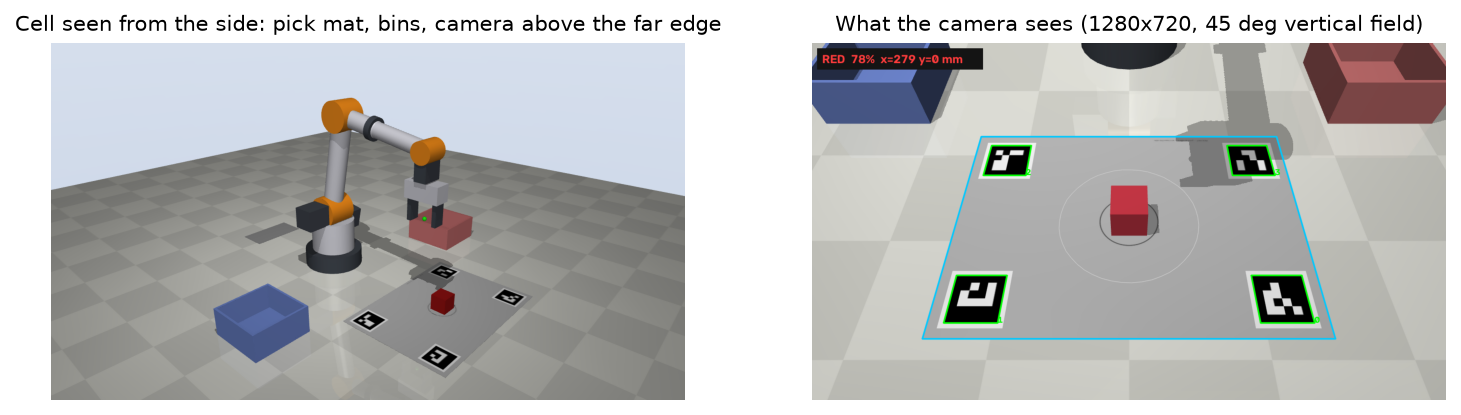
\includegraphics[width=\linewidth]{images/vision/e6_camera_placement.png}
  \caption{Camera placement. Left: the cell with the pick mat and the two bins. Right: the camera view, with the markers
  (green), the mat outline (blue) and the decision.}
  \label{fig:cv-placement}
\end{figure}

\subsection{Colour detection}

Each camera frame goes through these steps (Figure~\ref{fig:cv-steps}):
\begin{enumerate}
  \item Find the four markers on the mat.
  \item Straighten the mat into a top-down view, whatever the camera angle.
  \item White balance: scale each colour channel so that the grey mat looks neutral grey. This removes the effect of the
        colour and the brightness of the room light.
  \item Find the coloured blob around the cross. An object is present if the blob is larger than 250\,mm$^2$.
  \item Compute the hue (the colour angle) of the blob and compare it with the two stored values, red and blue. The answer
        is that colour if the difference is less than 28\,$^\circ$, otherwise \emph{unknown}.
  \item Repeat on five frames and keep the answer only if four agree.
\end{enumerate}

Before the run, each cube is placed on the cross and \texttt{python -m vision.calibrate colours} stores its hue from six
frames. \emph{Unknown} is a safe answer: the sequencer looks again or skips the object. A wrong guess would put a cube in
the wrong bin.

\begin{figure}[h]
  \centering
  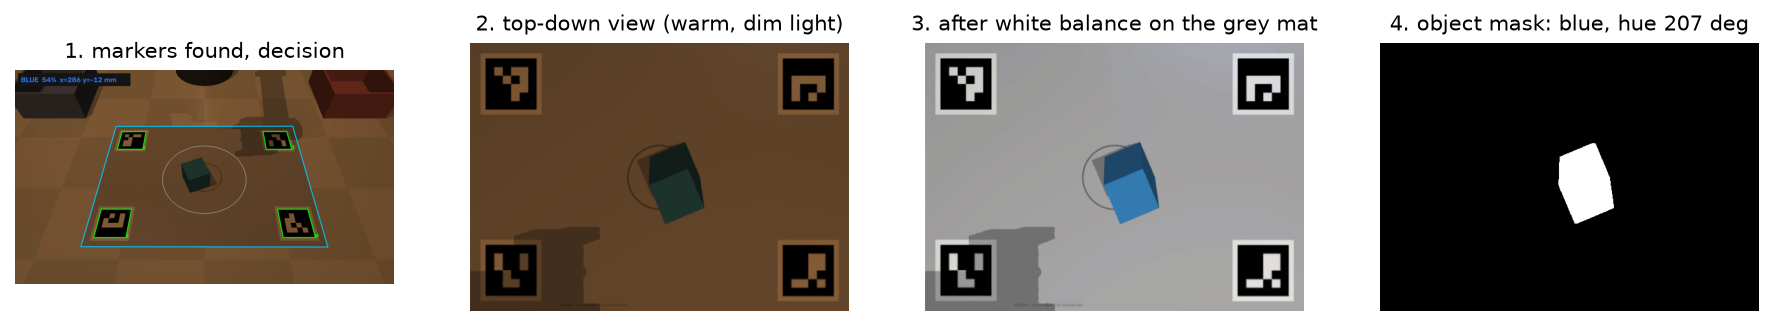
\includegraphics[width=\linewidth]{images/vision/e6_pipeline_steps.png}
  \caption{One frame under a warm, dim light: detection, top-down view, after white balance, and the object mask.}
  \label{fig:cv-steps}
\end{figure}

\subsection{Image to arm calibration}

The lens is measured once with a printed chessboard (OpenCV \texttt{calibrateCamera}). The camera position is then computed
in every frame from the four markers (\texttt{solvePnP}). Their positions in the arm's frame are known, because the mat is
taped with its cross on the pick spot and its edges along the arm's axes. If the camera is moved, nothing needs to be
calibrated again, as long as the mat is in view.

The camera also sees the sides of the cube, so the centre of the blob is slightly off the true centre. We correct this by
following the camera ray down to the height $h$ of the cube centre, with $\mathbf{c}$ the camera position,
$\mathbf{p}_0$ the blob centre on the table, and $\mathbf{p}$ the object centre:
\[
  \mathbf{p} = \mathbf{c} + (\mathbf{p}_0 - \mathbf{c})\,\frac{c_z - h}{c_z}.
\]
This gives goal G2. For G3, the cube lies on the table, so its height is known: $z = 15$\,mm for a 30\,mm cube. A single
camera cannot measure the height of an object of unknown size; that would need a depth camera.

\subsection{Results}
\label{sec:cv-results}

No hardware exists yet, so the plan was tested on 600 frames from a simulated camera at the planned position, with image noise
and JPEG compression added. In each frame the object was chosen at random (red, blue, green, yellow, or no object) and placed
up to 20\,mm off the cross. The light changed from 0.35 to 1.5 times the normal brightness and from warm (2700\,K) to cold
(8000\,K). Green and yellow objects must be refused. Table~\ref{tab:cv-results} compares our method with the same method
without the white balance.

\begin{table}[h]
  \centering
  \caption{Results on 600 simulated frames.}
  \label{tab:cv-results}
  \begin{tabular}{@{}lrr@{}}
    \toprule
    & With white balance & Without \\ \midrule
    Correct answers & 100\,\% & 81.7\,\% \\
    Red or blue cube sent to the wrong bin & 0 of 477 & 32 of 477 \\
    Green or yellow cube sent to a bin & 0 & 0 \\
    Empty mat reported as an object & 0 & 28 \\ \bottomrule
  \end{tabular}
\end{table}

Without the white balance, a warm light changes the measured hue of the objects (Figure~\ref{fig:cv-hue}) and colours the
whole mat, which is then mistaken for an object. With it, every object stays close to its stored colour.
The markers were found in all 600 frames. The object centre was found with a median error of 1.6\,mm and a worst case of
2.2\,mm (Figure~\ref{fig:cv-position}); without the height correction the median error is 13.4\,mm.
Figure~\ref{fig:cv-examples} shows some of the frames.

\begin{figure}[h]
  \centering
  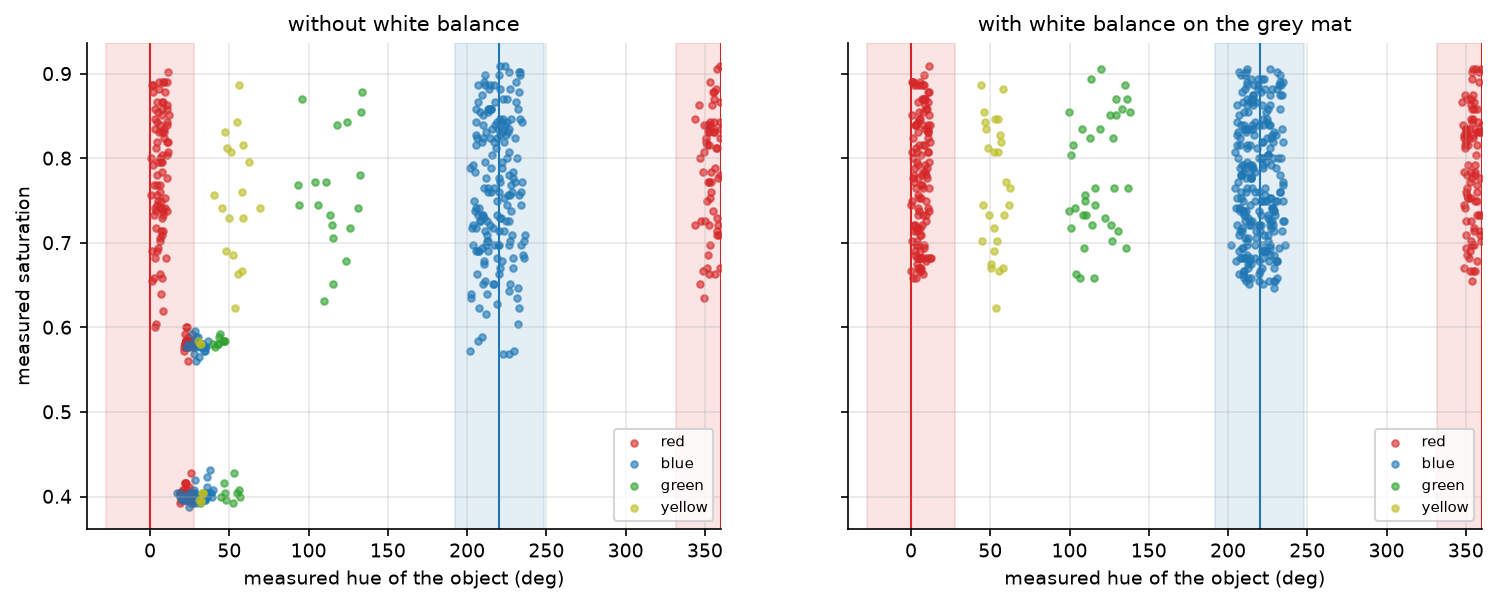
\includegraphics[width=\linewidth]{images/vision/e6_hue_scatter.png}
  \caption{Measured hue and saturation of every object, without (left) and with (right) the white balance. The shaded
  bands are the accepted ranges of red and blue.}
  \label{fig:cv-hue}
\end{figure}

\begin{figure}[h]
  \centering
  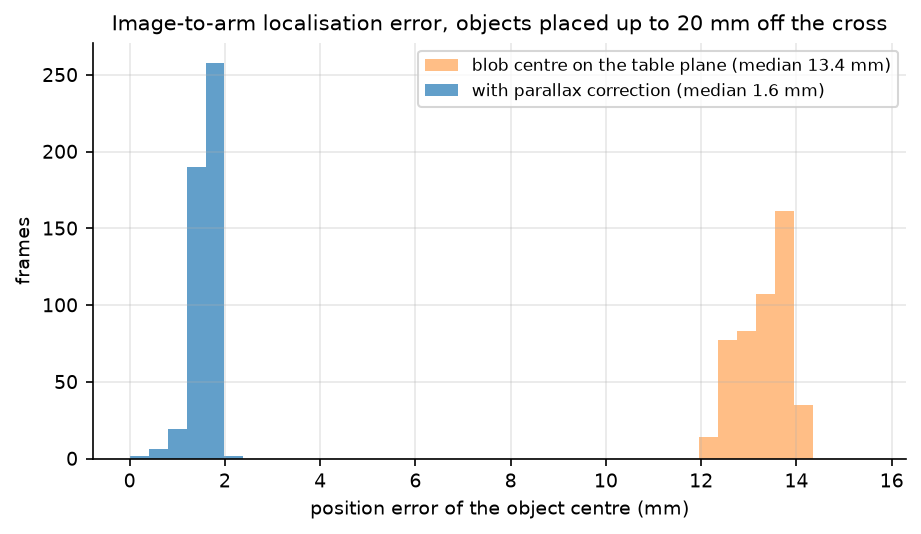
\includegraphics[width=0.75\linewidth]{images/vision/e6_position_error.png}
  \caption{Error of the object position, with and without the height correction.}
  \label{fig:cv-position}
\end{figure}

\begin{figure}[h]
  \centering
  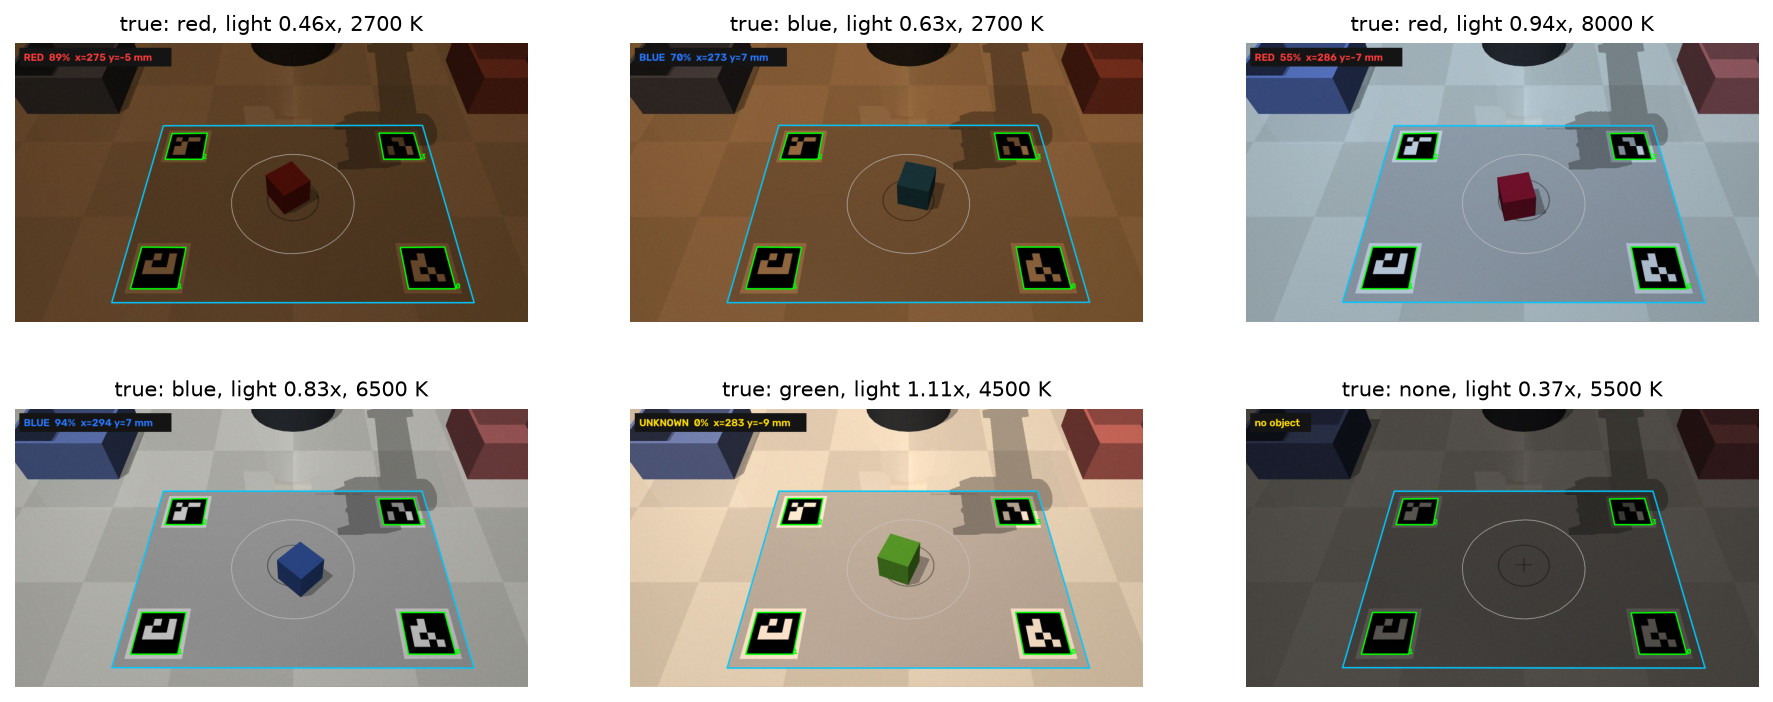
\includegraphics[width=\linewidth]{images/vision/e6_examples.png}
  \caption{Answers on test frames under different lights.}
  \label{fig:cv-examples}
\end{figure}

These are simulated images: they test the method, not the webcam. Real lens distortion, automatic exposure and shiny
surfaces are not included, and the real colours of the cubes are not known yet. In the build phase the test will be repeated
with the real camera and cubes, 20 cycles per colour (requirement R4).

% ---------------------------------------------------------------------------
% Suggested changes elsewhere in the book
% ---------------------------------------------------------------------------
% 1.3.2 Motion strategy, cycle: read the colour BEFORE the grasp, while the arm waits at the ready pose:
%   "A cycle is: wait at the ready pose until the camera sees a cube, read its colour and position, move above it,
%    descend, close the gripper, lift, move to the bin, open, return."
% 1.3.3 Algorithms, colour classification:
%   "A fixed webcam views the pick location on a printed grey mat with four ArUco markers. The markers give the camera pose,
%    the grey mat gives the white balance, and the cube is classified by its hue against two stored values, with a
%    rejection band for unknown colours and a vote over five frames (Section 6)."
% 1.6 Bill of materials, camera line:
%   "1  USB webcam 1280x720 + printed A4 pick mat + LED light   colour and position   team"
% 1.7 Risks, colour line, mitigation:
%   "White balance on the grey mat, calibration in place, unknown colours refused; tested from 2700 K to 8000 K (Section 6.4)."
